\section{Principal Component Analysis} 
  
  We can think of PCA doing two things. First, it is a dimensionality-reduction algorithm where it takes samples $x \in \mathbb{R}^d$ and projects them into some smaller subspace $\mathcal{L}$ of dimension $k$. Second, it identifies an orthonormal basis of $\mathcal{L}$ that act as uncorrelated low-dimensional features. Because the projection map is linear and we are working in a lower-dimensional subspace, these new basis vectors are linear combinations of the original basis, which may reduce redundancy. Furthermore, by approximately modeling the original $x$ as a linear combination of these features, we are able to get a more parsimonious representation. 

  To begin, let $X$ be the 

  To begin with some motivation, let a linear map $A: \mathbb{R}^D \rightarrow \mathbb{R}^D$ be full rank, which maps some set of $n$ data points to the space of features. Then it is injective, and therefore for all data $x \in \mathbb{R}^D$ there exists a feature vector $z \in \mathbb{R}^D$ such that $z = Ax$. Generally, real-world data does not span the full space of $D$ dimensions.\footnote{The \textit{manifold hypothesis} that real-world data in high-dimensions actually lies on a lower-dimensional manifold. } In fact, if we further assume that the data lies in a linear subspace, we want to compress it into a lower-dimensional vector such that the covariates in this lower dimensional space are also orthogonal, i.e. uncorrelated. We tackle both problems in 2 steps. 
  \begin{enumerate}
    \item To compress this representation, we can take a data point $x \in \mathbb{R}^D$ and \textit{approximate} it as a point $\hat{x} \in L_k$ for some $k$-dimensional subspace $L_k \subset \mathbb{R}^d$ (say that this is done with some function $P: \mathbb{R}^D \rightarrow L_k \subset \mathbb{R}^D$). 
    \item After this projection, we then want to extract the $k$ features such that they are \textit{orthogonal} (i.e. no correlation). This is done with a simple change of basis, which we denote $T: L_k \rightarrow \mathbb{R}^k$, giving us $\hat{z} = T \hat{x} = T (P(x))$. We can invert this map $T^{-1} : \mathbb{R}^k \rightarrow L_k$ to go from the orthogonalized compressed version $\hat{z}$ to the approximate full version $\hat{x}$.
  \end{enumerate}

\subsection{Principal Subspace as an L2 Distance Minimizer}

  We are done! But which subspace do we choose? Let's formalize what the optimal subspace should be. 

  \begin{definition}[Principal Subspace]
    Let $x \sim X \in \mathbb{R}^d$, with its normalized $\tilde{x} = x - \mathbb{E}[x]$, and $\mathcal{L}_k$ denote all $k$-dimensional linear subspaces of $\mathbb{R}^n$. The \textbf{$k$th principal subspace} is defined as 
    \begin{equation}
      \ell_k = \argmin_{\ell \in \mathcal{L}_k} \mathbb{E}_{\Tilde{x}} \big( \min_{y \in \ell} ||\Tilde{x} - y||^2 \big)
    \end{equation}
  \end{definition}

  To parse this, let's fix a subspace $\ell$. Then, the normalized data $\Tilde{x}$ is a random vector and the minimum distance of $\Tilde{x}$ onto the subspace $\ell$ is the inner min term. Taking the expectation of that gives us the expected distance of the data onto the subspace. The principal subspace is the subspace that minimizes this expected distance. The dimension reduced version of $x$ is then $P_k (x) = \mu + \mathrm{proj}_{\ell_k} x$. 

  We can see that by definition the properties of the principal subspace allows us to construct the best approximation of the points in a lower-dimensional subspace. This seems like a hard optimization problem, but it turns out that the theorem gives a simple solution. Note that we need to do 3 things: 
  \begin{enumerate}
    \item Find such a subspace $\mathcal{L}_k \subset \mathbb{R}^D$. 
    \item Find the projection $P_k: \mathbb{R}^D \rightarrow \mathcal{L}_k \subset \mathbb{R}^D$. Note that by definition of the principal subspace $P_k$ should be an \textit{orthogonal} projection. 
    \item Find the bijection $T_k: \mathcal{L}_k \rightarrow \mathbb{R}^k$. 
  \end{enumerate}

\subsection{Principal Components as a Greedy Variance Maximization Approach}

  \begin{figure}
    \centering
    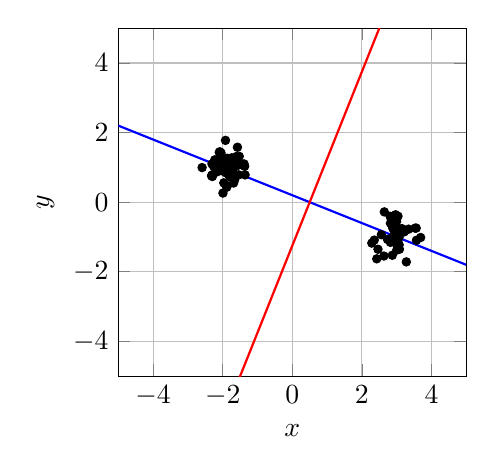
\begin{tikzpicture}
      \begin{axis}[
        xlabel={$x$}, ylabel={$y$},
        axis equal,
        xmin=-5, xmax=5,
        ymin=-5, ymax=5,
        grid=both,
        width=6cm, height=6cm
      ]
      
      \foreach \i in {1,...,50} {
        \pgfmathsetmacro\x{-2 + 0.8*rnd*cos(360*rnd)}
        \pgfmathsetmacro\y{1 + 0.8*rnd*sin(360*rnd)}
        \addplot[only marks, mark=*, mark size=1.5pt, color=black] coordinates {(\x,\y)};
      }
      
      \foreach \i in {1,...,50} {
        \pgfmathsetmacro\x{3 + 0.8*rnd*cos(360*rnd)}
        \pgfmathsetmacro\y{-1 + 0.8*rnd*sin(360*rnd)}
        \addplot[only marks, mark=*, mark size=1.5pt, color=black] coordinates {(\x,\y)};
      }

      % Line from (-2,1) to (3,-1): slope -2/5
      \addplot[thick, blue, domain=-5:5, samples=2] {-0.4*(x + 2) + 1};

      % Perpendicular line through midpoint (0.5, 0), slope 5/2
      \addplot[thick, red, domain=-5:5, samples=2] {2.5*(x - 0.5)};
      \end{axis}
    \end{tikzpicture}
    \caption{Projecting the dataset onto the blue line seems to retain more variance than projecting onto the red line.}
  \end{figure}

\subsection{Solving PCs with Singular Value Decomposition}

  It turns out that we can solve all three problems with the singular value decomposition. 

  \begin{theorem}[Construction of the kth Principle Subspace] 
    Given covariates $x^{(1)}, \ldots, x^{(n)} \in \mathbb{R}^{d}$, let $X \in \mathbb{R}^{n \times d}$ be our random matrix representing our data, and its normalized form to $\Tilde{X} = X - \mu$. We take the SVD of it. 
    \begin{equation}
      \Tilde{X} = U \Sigma V^T
    \end{equation}
    where $U \in U(n) \subset \mathbb{R}^{n \times n}, V \in U(d) \subset \mathbb{R}^{d \times d}$ are orthogonal and $\Sigma \in \mathbb{R}^{n \times d}$ is diagonal that represents the singular values of $X$ in decreasing order\footnote{We can make it decreasing by permuting the rows/columns of the unitary matrices $U, V$.}. The columns of $V$ (rows of $V^T$) denoted $v_1, \ldots, v_d$ are called the \textbf{principal axes} and the columns of $U\Sigma$ are called the \textbf{principal components}. 
    \begin{enumerate}
      \item Then $\ell_k = \mathrm{span}\{v_1, \ldots, v_k\} \subset \mathbb{R}^d$, i.e. is the subspace spanned by the columns of $V$. By shifting it by $\mu$, $\mu + \ell_k$ is the best affine subspace approximation of the $x_i$'s. 

      \item The projection $P$ is defined 
      \begin{equation}
        \hat{x} = P_k (x) = \mu + \sum_{j=1}^k \langle x - \mu, v_j \rangle \, v_j = \sum_{j=1}^k \proj_{v_j} (x - \mu) = \mu + \proj_{\ell_k} (x - \mu)
      \end{equation}
      where we can rewrite it as the projection operator since the $v_j$'s are orthonormal. 

    \item The change of basis $T$ is defined with the mapping $\hat{x} \in \mathcal{L}_k \mapsto \sigma_j v_j \in \mathcal{L}_k$. Note that the $v_j$'s form an orthogonal basis of $\mathcal{L}_k$. 
    \end{enumerate} 
    Now let $V_k \in \mathbb{R}^{d \times k}$ represent the first $k$ columns of $V$ (aka first $k$ principal axes), $U_k \in \mathbb{R}^{n \times k}$ represent the first $k$ columns of $U$, and $\Sigma_k \in \mathbb{R}^{k \times k}$ represent the upper-left $k \times k$ matrix of $\Sigma$.\footnote{Note that $V^T$, which was originally surjective, is now just injective.} The product $U_k \Sigma_k$ represents the matrix containing the first $k$ principal components. The matrix $\Tilde{X}_k = U_k \Sigma_k V^T$, which is the low-rank approximation of $\Tilde{X}$, is called the \textbf{denoised matrix} of $\Tilde{X}$. 
  \end{theorem}
  \begin{proof}
    For notational convenience let $X = \Tilde{X}$. We see that 
    \begin{equation}
      X^T X =  V \Sigma^T \Sigma V^T
    \end{equation}
    Note that $X \neq V \Sigma^T$ in general. Now let $v_1, \ldots, v_d$ be the columns of $V$. Then 
    \begin{equation}
      X^T X [v_1, \ldots, v_d] = X^T X V = V \Sigma^T \Sigma = [\sigma_1^2 v_1, \ldots, \sigma_d^2 v_d]
    \end{equation}
    Therefore, we can see that the way $X^T X$ acts on $V$ That the $v_i$'s are the eigenvectors of $X^T X$, with $\sigma_i^2$ the associated eigenvalues. 
  \end{proof}

  Let's take a few moments to appreciate what $U$ and $V$ really represent. In some sense, $U_k \in \mathbb{R}^{n \times k}$ can be considered the dimension-reduced form of $\Tilde{X} \in \mathbb{R}^{n \times d}$. To see why consider the following. Let's label the \textit{rows} of $U_k$ as $u^{(1)}, \ldots, u^{(n)} \in \mathbb{R}^k$. By transposing the equation of the denoised matrix, we get $\Tilde{X}_k^T = V_k \Sigma_k U_k^T$, and so 
  \begin{equation}
    x^{(i)} - \mu = V_k \Sigma_k u^{(i)}
  \end{equation}
  for $i = 1, \ldots, n$. As an immediate consequence, since $T^{-1}$ maps $e_j$ to $\sigma_j v_j$, we can interpret $U_k \Sigma_k V_k^T$ with the decomposition 
  \begin{center}
    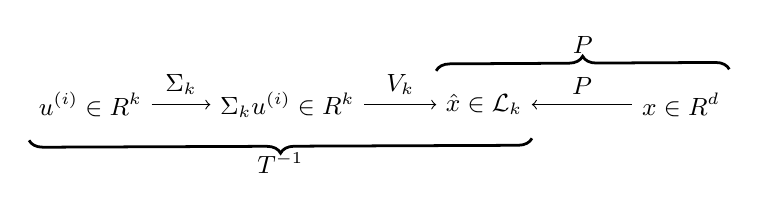
\begin{tikzpicture}[
      node distance=2.5cm,
      every node/.style={font=\small}
    ]
      % Nodes
      \node (vj) {$u^{(i)} \in \mathbb{R}^k$};
      \node[right of=vj] (sigmavj) {$\Sigma_k u^{(i)} \in \mathbb{R}^k$};
      \node[right of=sigmavj] (xhat) {$\hat{x} \in \mathcal{L}_k$};
      \node[right of=xhat] (x) {$x \in \mathbb{R}^d$};
      
      % Arrows
      \draw[->] (vj) -- node[above] {$\Sigma_k$} (sigmavj);
      \draw[->] (sigmavj) -- node[above] {$V_k$} (xhat);
      \draw[<-] (xhat) -- node[above] {$P$} (x);
      
      % Braces with increased thickness
      \draw[line width=1pt] [decoration={brace,mirror,raise=5pt,amplitude=5pt},decorate] (vj.south west) -- 
            node[below=6pt] {$T^{-1}$} (xhat.south east);
      \draw[line width=1pt] [decoration={brace,raise=5pt,amplitude=5pt},decorate] (xhat.north west) -- 
            node[above=7pt] {$P$} (x.north east);
    \end{tikzpicture}
  \end{center}

  This is very revealing. To embed the low-rank $u^{(i)}$ representation, it must go through some scaling $\Sigma_k$ followed by the injective map $V_k$. Now let's interpret $V_k$ and consider its \textit{columns}, labeled $v_1, \ldots, v_k \in \mathbb{R}^d$. These represent the basis vectors that span the subspace $\mathcal{L}_k$, i.e. the upscaled features in the higher-dimensional space. Therefore, $V_k$ represents the injection $e_i \in \mathbb{R}^k \mapsto v_i \in \mathcal{L}_k \subset \mathbb{R}^d$. This means that if we would like to pick a point with some combination of these features, we are really picking a point 
  \begin{equation}
    z = \sum_i z_i v_i \in \mathcal{L}_k
  \end{equation}

  \begin{algo}[Fitting] 
    Given a dataset $X \in \mathbb{R}^{n \times d}$, let us denote the rows as $x_i$, and say that we are looking for a subspace of dimension $k$. 
    \begin{enumerate}
      \item Compute the mean 
      \begin{equation}
        \mu = \frac{1}{n} \sum_{i=1}^n x_i  \in \mathbb{R}^d
      \end{equation} 

      \item Standardize the data $\Tilde{X} = X - \mu$, i.e. $\Tilde{x}_i = x_i - \mu$.  

      \item Compute the SVD $\Tilde{X} = U \Sigma V^T$.

      \item Compute the submatrices $V_k \in \mathbb{R}^{k \times k}$ and $\Sigma_k \in \mathbb{R}^{D \times k}$. 

      \item Define the projection operator $P_k (x) = \mu + \sum_{j=1}^k \langle x - \mu, v_j \rangle \, v_j$, the change of basis operator $T$, and the embedding operator $T^{-1} (z) = \mu + V_k \Sigma_k z$. 
    \end{enumerate} 
    A demonstration is done \href{code/pca.html}{here}.
  \end{algo}

  \begin{example}[Eigenfaces]
    In 1991, Turk and Pentland presented an eigenface method of face recognition by taking the low-rank approximation of a dataset of face images. 

    \begin{figure}[H]
      \centering 
      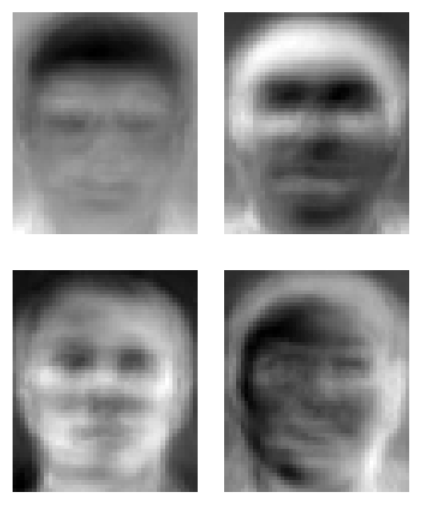
\includegraphics[scale=0.3]{img/eigenfaces.png}
      \caption{Some eigenfaces from AT\&T Labs. } 
      \label{fig:eigenfaces}
    \end{figure}
  \end{example}

  Now a question arises: how do we know that this sample decomposition is a good approximation to the true decomposition? It comes from the fact that the sample covariance $\hat{\Sigma}$ is a good approximation of the true covariance $\Sigma$, which we will later prove using concentration of measure. 

  \begin{theorem}[Risk]
    The risk satisfies 
    \begin{equation}
      R(k) = \mathbb{E}[|| x - P_k (x) ||^2 ] = \sum_{j=k+1}^D \lambda_j 
    \end{equation}
  \end{theorem}

  It is essential that you plot the spectrum in decreasing order. This allows you to analyze how well PCA is working. People often use the ``elbow'' technique to determine where to choose $K$, and we value 
  \begin{equation}
    \frac{\sum_{j=1}^k \lambda_j}{\sum_{j=1}^d \lambda_j} 
  \end{equation}
  accounts for the \textbf{variance explained}, which should be high with $K$ low. If you have to go out to dimension $K=50$ to explain $90\%$ of the variance, then PCA is not working. It may not work because of many reasons, such as there being nonlinear structure within the data. 

  It turns out that the elements of $\hat{\Sigma}$ are close entry-wise to those of $\Sigma$. But if this is true, then does it mean that the eigenvalues of the sample covariance matrix are close to the true eigenvalues of the covariance matrix? It turns out that the answer is no, and we need a proper metric to satisfy this assumption. The metric, as we can guess from linear algebra, is the operator norm, and we will show some results from matrix perturbation theory. 

  \begin{lemma}[]
    It turns out that 
    \begin{equation}
      ||\hat{\Sigma} - \Sigma|| = O_p \bigg( \frac{1}{\sqrt{n}} \bigg)
    \end{equation}
    where $|| \cdot ||$ is the operator norm. 
  \end{lemma}

  \begin{theorem}[Weyl's Theorem]
    If $\hat{\Sigma}$ and $\Sigma$ are close in the operator norm, then their eigenvalues are close. 
    \begin{equation}
      ||\hat{\Sigma} - \Sigma|| = O_p \bigg( \frac{1}{\sqrt{n}} \bigg) \implies |\hat{\lambda}_j - \lambda_j| = O_p \bigg( \frac{1}{\sqrt{n}} \bigg) 
    \end{equation}
  \end{theorem}

  This only talks about their eigenvalues, but this does not necessarily imply that the eigenvalues are close. We need an extra condition. 

  \begin{theorem}[David-Kahan Theorem]
    If $\hat{\Sigma}$ and $\Sigma$ are close in the operator norm, and if the eigenvectors of $\Sigma$ are well-conditioned, then the eigenvectors of $\hat{\Sigma}$ are close to the eigenvectors of $\Sigma$. More specifically, 
    \begin{equation}
      ||\hat{v}_j - v_j|| \leq \frac{2^{3/2} ||\hat{\Sigma} - \Sigma||}{\lambda_j - \lambda_{j+1}}
    \end{equation}
  \end{theorem}

